\begin{frame}[fragile]{Conclusion}
\begin{columns}[c]
    \begin{column}{0.50\textwidth}
    \begin{itemize}
        \item Undefined behaviour in compiler IR \textbf{enables} desirable optimizations
        \item Having \textbf{two distinct} semantics for deferred UB was a source of historical bugs
        \item The \texttt{freeze} instruction is now part of LLVM, so \texttt{undef} is now \textbf{deprecated}
    \end{itemize}
    \end{column}
    \begin{column}{0.54\textwidth}
        \begin{figure}
            \centering
            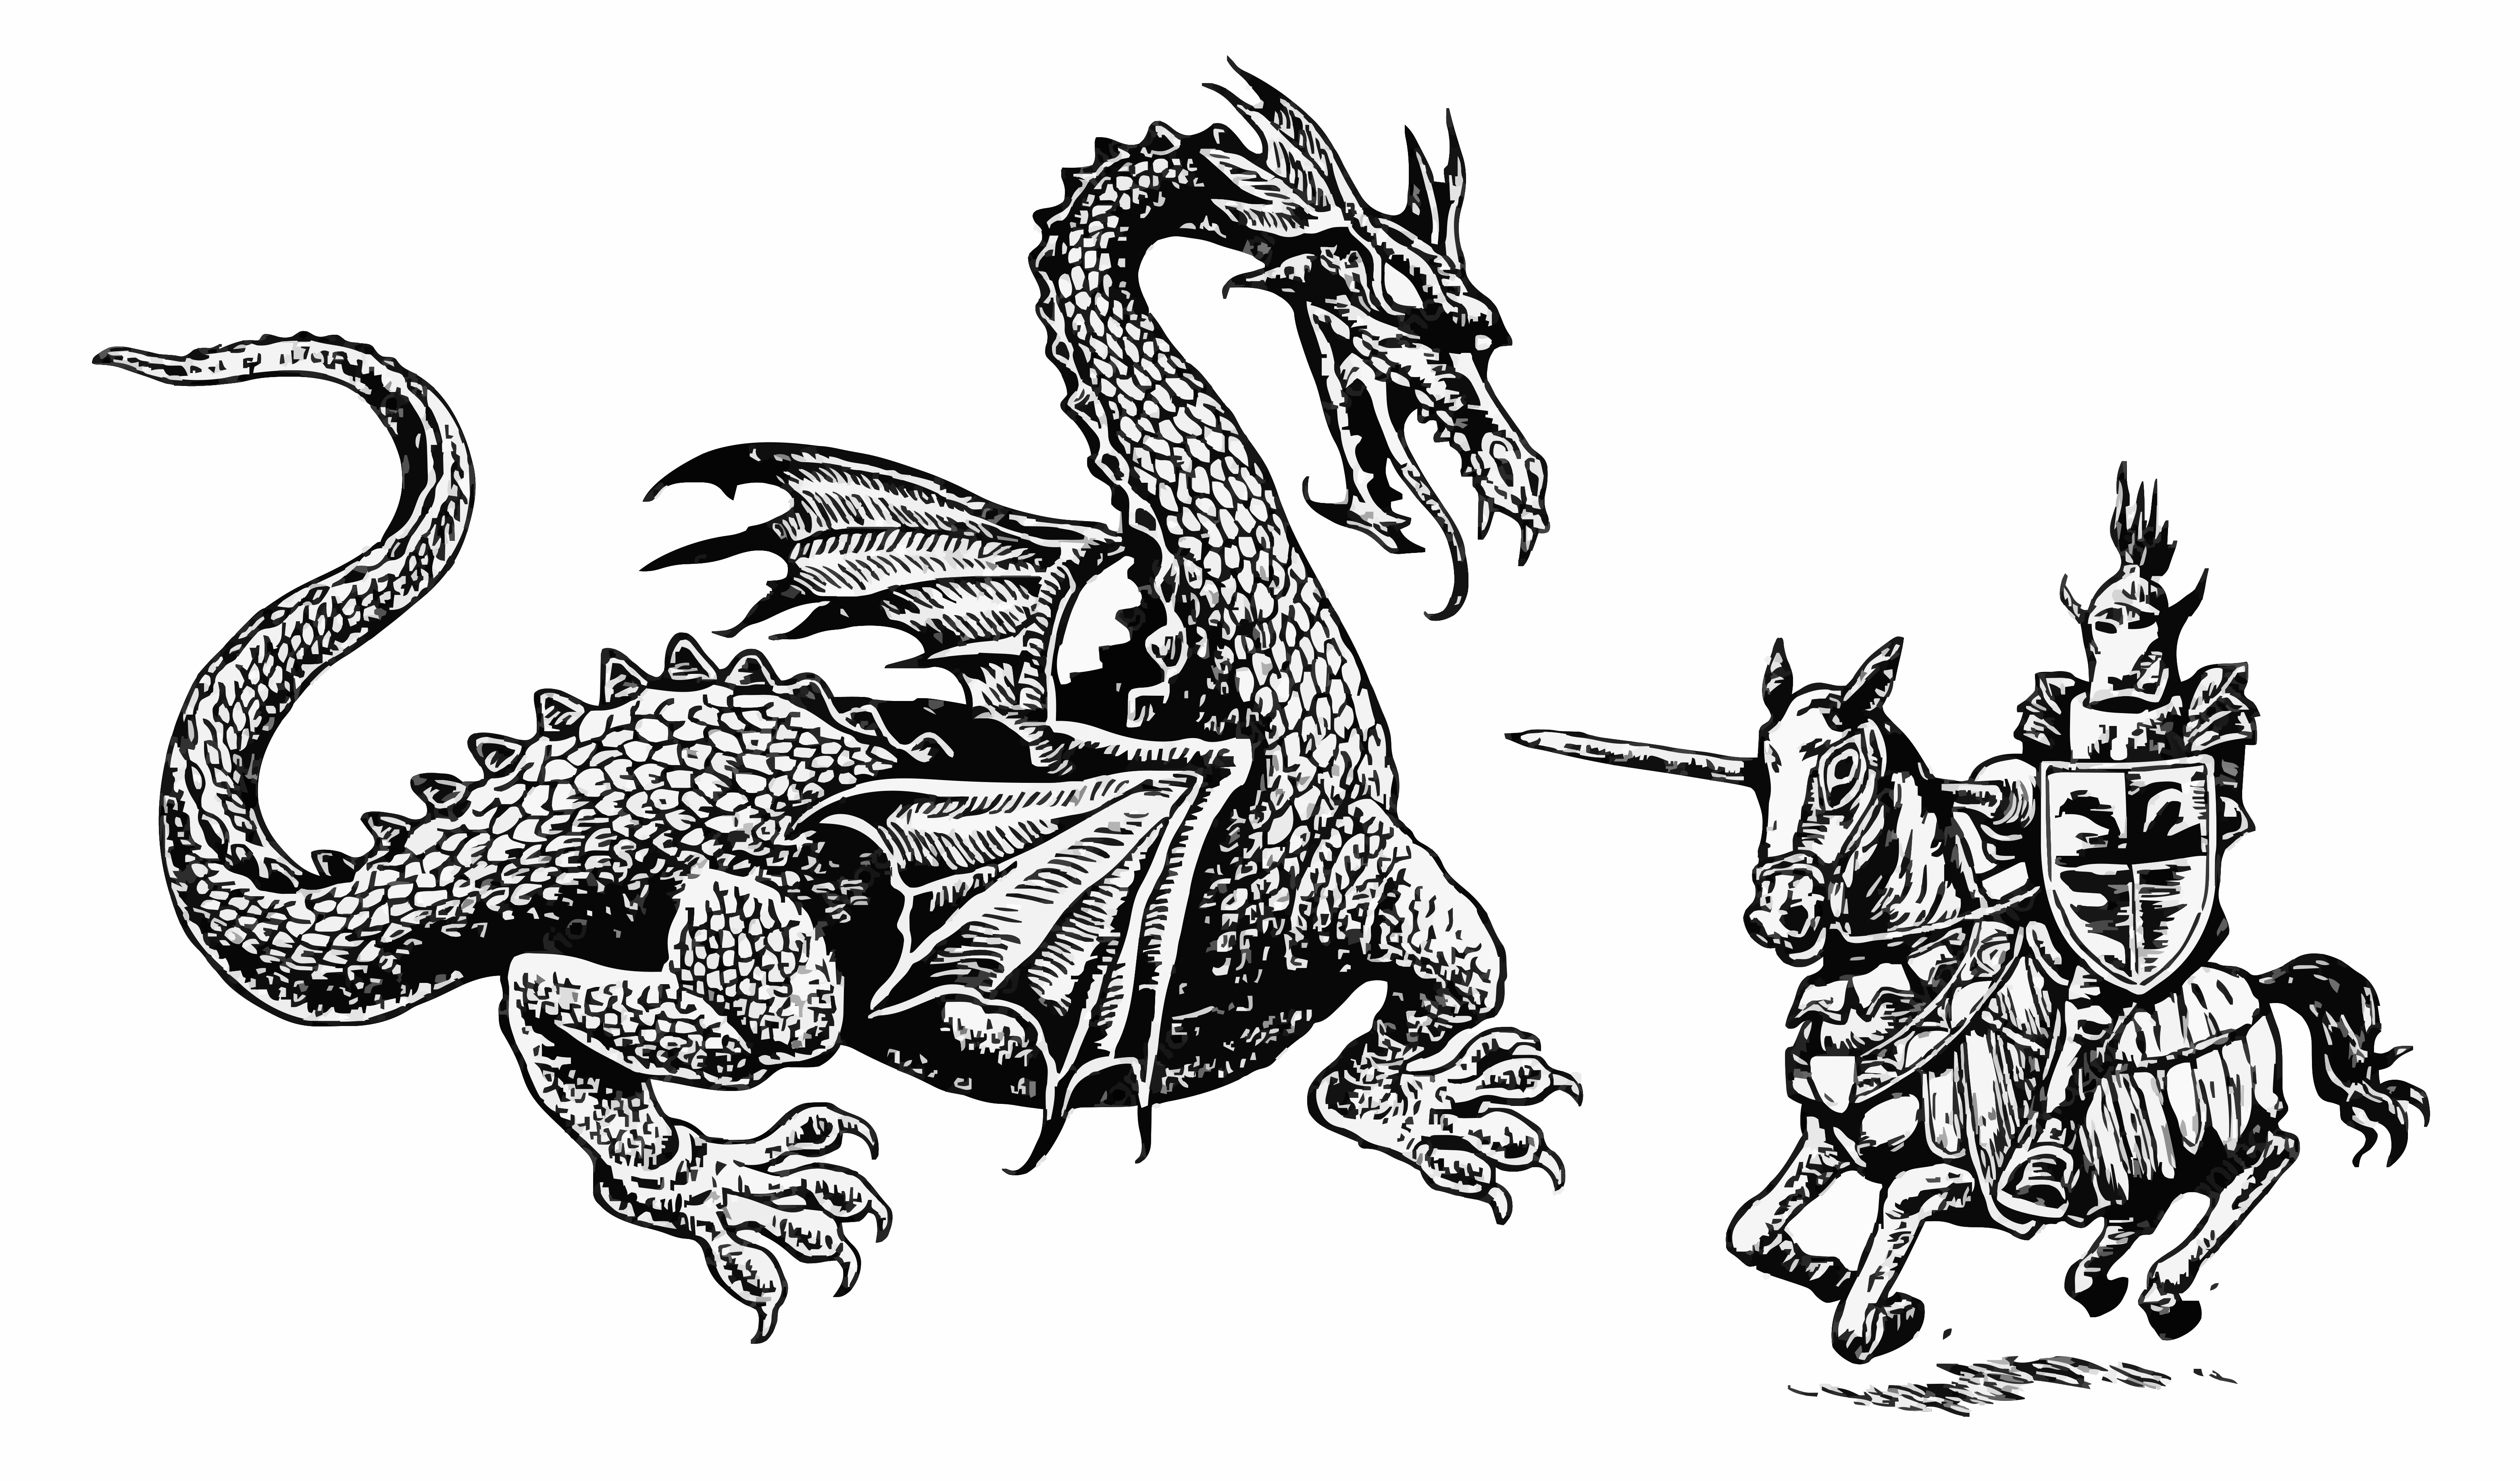
\includegraphics[width=1.05\textwidth]{images/dragon-knight.png}
        \end{figure}
    \end{column}
\end{columns}

\pdfpcnote{
Close with the three takeaways: 

1. UB is necessary for desirable optimizations
2. Having two distinct deferred-UB mechanisms was a historic source of bugs
3. The freeze instruction is the clean solution now adopted by LLVM with undef deprecated. 
Leave time for questions — likely topics are the undef/poison distinction, why phi and
select are exceptions to poison propagation, and why freeze cannot be duplicated
or sunk into loops.
}

\end{frame}
